% !TEX root = ../Main.tex
\documentclass[../Main.tex]{subfiles}
\begin{document}

\subsection{Virtuelle Maschine}

Eine virtuelle Maschine (VM) ist eine Umgebung in der CPU, Speicher, Netzwerkschnittstelle und Storage von einem physischen
Hardware-System bereitgestellt werden und durch einen Hypervisor (Software) provisioniert und getrennt werden \citep{VirtuelleMaschine}.

Kernel-based Virtual Machine (KVM) ist eine Open-Source Virtualisierungstechnologie die im Linux-Kernel integriert ist. Dadurch kann ein Hypervisor mehrere isolierte
virtuelle Umgebungen ausführen. KVM wird von allen gängigen Linux-Distributionen und X86-Hardware unterstützt \citep{KVM}.

\subsection{Ansible}

Ansible ist ein Softwaretool zur plattformübergreifenden Automatisierung von Abläufen.
Primär wird es von IT Experten verwendet um das Ausrollen von Applikationen, Updates oder Konfigurationen zu vereinfachen, dabei ist
kein Agent auf den Ziel-Computern notwendig.
Die Automatisierung wird in Form von Skripten geschrieben, was die Versionierung erleichtert und Anwenderfreundlich ist. Dies sind einfache Dateien im YAML-Format und das ausführen idempotent.
Das bedeutet, dass ein mehrfaches Ausführen eines Playbooks keine negativen Effekte hat wenn das System bereits korrekt konfiguriert ist \citep{Ansible}.

\subsection{OpenStack}

OpenStack ist eine Cloud Software die eine gro{\ss}e Anzahl von Compute-, Storage-, und Netzwerkressourcen
verwaltet. Durch eine Web-Anwendung kann die Cloud verwaltet und Ressourcen provisioniert werden \citep{OpenStack}.

OpenStack besteht aus einzelnen Projekten die bestimmte Dienste wie Computing, Networking oder Storage anbieten und
API Schnittstellen (Application Programming Interface) zur Verfügung stellen \citep{OpenstackComponents}.

OpenStack wurde im Juli 2010 gemeinsam von RackSpace und NASA als Open-Source Projekt vorgestellt um NASA's Nebula Platform und Rackspace's Cloud Dateispeicherdienst zu vereinen. Mittlerweile beteiligen sich viele
namenhafte Firmen an der Weiterentwicklung der einzelnen Projekte \citep{WhatIsOpenStack}.

Die Projekte sind modular aufgebaut und interagieren untereinander über APIs. Zu den wichtigsten Projekten zählen \citep{WhatIsOpenStack}:
\begin{itemize}
    \item[] \textbf{Nova:} Nova ist der primäre Compute-Dienst und für das Planen, Erstellen und Löschen von virtuellen Maschinen zuständig. Nova unterstützt neben dem KVM-Hypervisor auch Hyper-V, VMware ESXi oder Xen.
    \item[] \textbf{Glance:} Glance ist ein Abbild-Dienst der für das Hochladen, die Verwaltung und das Löschen von Abbildern zuständig ist. Glance unterstützt unter anderem Ceph, NFS oder Swift als Backend \citep{OpenStackGlanceStores}.
    \item[] \textbf{Neutron:} Neutron verwaltet die Netzwerkinfrastruktur und stellt die Verbindung zwischen Instanzen sicher. Dazu zählen zum Beispiel Software-Defined-Networking (SDN) Technologien wie Open vSwitch (OVS) oder Open Virtual Network (OVN).
    \item[] \textbf{Cinder:} Cinder ist eine Block Storage Komponente und erstellt, verwaltet und löscht persistente Block Devices. Diese können in die Instanzen eingehängt werden.
    \item[] \textbf{Swift:} Swift ist eine weitere Storage Komponente das hochverfügbaren Speicher ähnlich wie Amazon S3 anbietet. Dabei können ungeordnete Daten-Objekte über REST-APIs verwaltet werden.
    \item[] \textbf{Keystone:} Keystone stellt Authentifizierungs- und Autorisierungsdienste für Nutzer bereit. Daneben ist auch eine Anbindung an externe Identitätsdienste wie LDAP oder Active Directory möglich.
\end{itemize}

Weitere Dienste sind unter anderem Horizon (Web Frontend), Designate (DNS Dienst), Ironic (Bare Metal) oder Ceilometer (Monitoring) \citep{OpenStackProjects}.

OpenStack Kolla ist ein weiteres Projekt welches Container und Tools zum Ausrollen einer OpenStack Cloud bereitstellt. Kolla-Ansible ist dabei ein Unterprojekt, dass das
automatische Ausrollen der Container mit Ansible erlaubt. Dies ist für Produktive-, aber auch für Entwicklungsumgebungen vom Vorteil, da es ein reproduzierbares und automatisches Deployment ermöglicht \citep{OpenStackKolla}.

\begin{figure}[h]
    \centering
    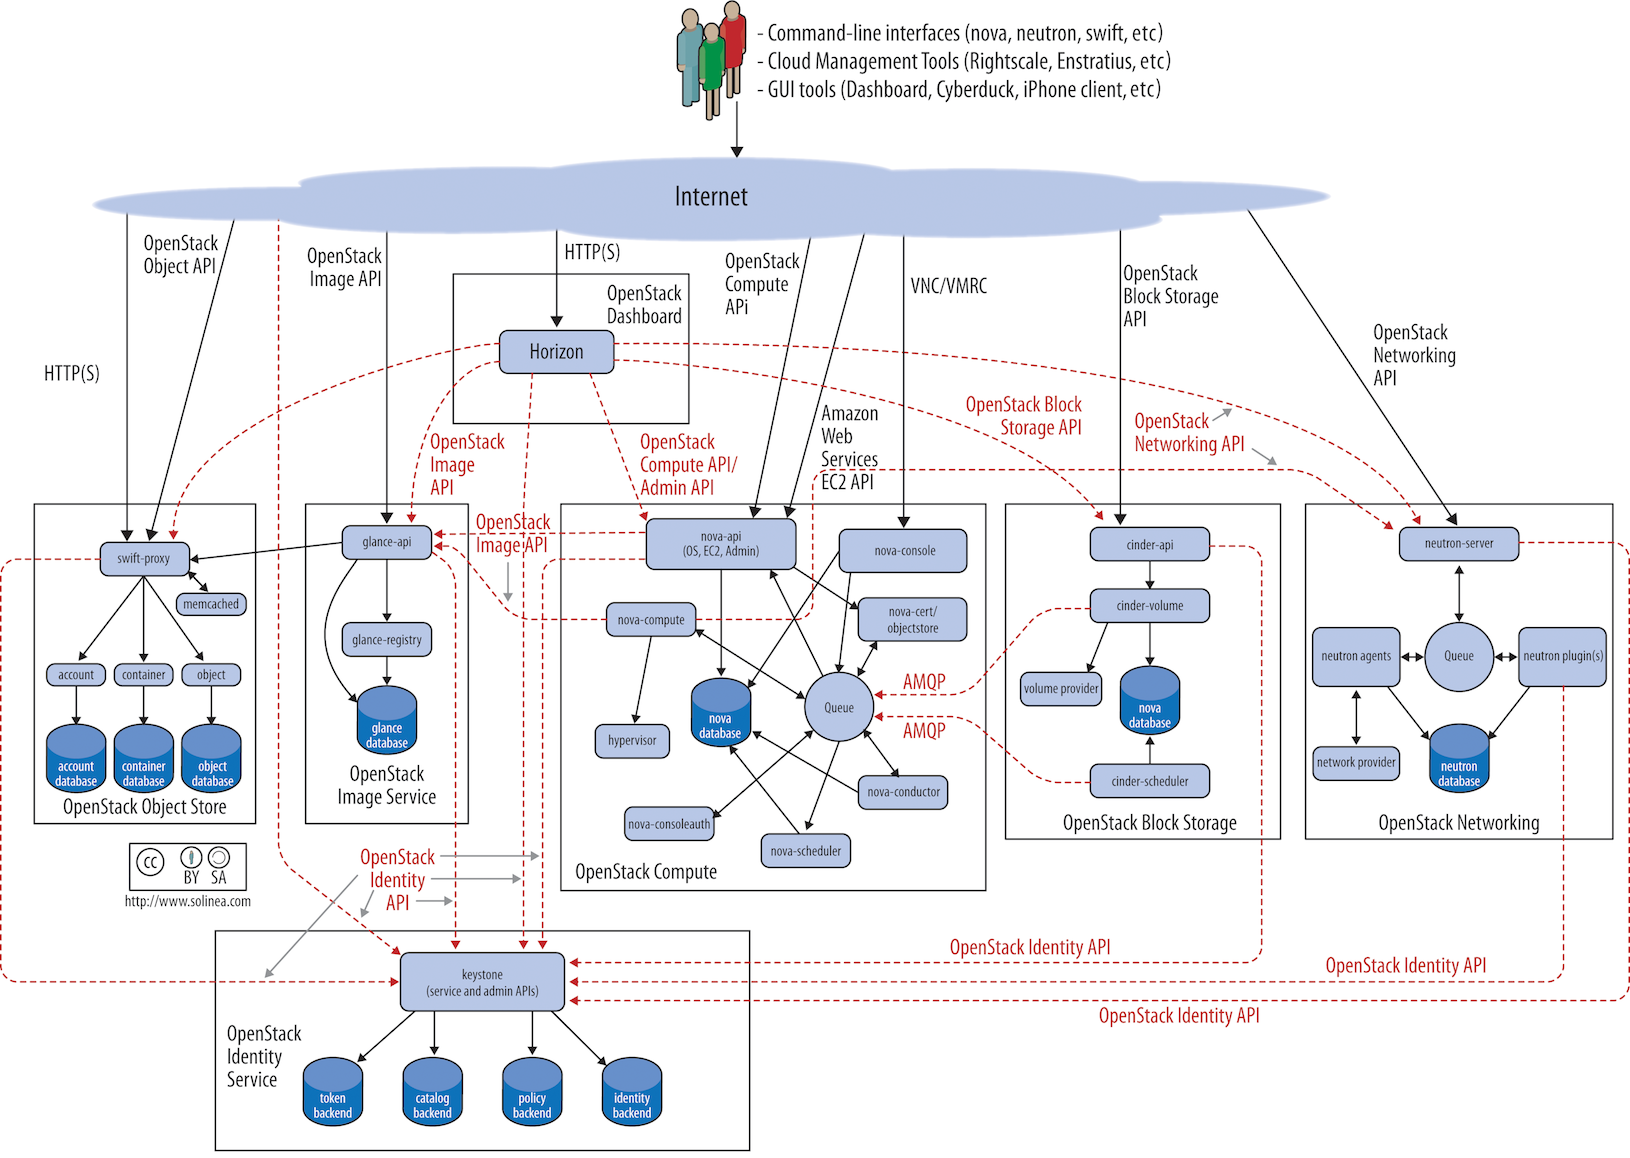
\includegraphics[width=0.9\columnwidth]{Images/OpenstackArchitecture.png}
    \caption{OpenStack Architektur \citep{OpenStackArchitecture}}
\end{figure}

\subsection{Docker}
Docker ist eine offene Plattform für die Entwicklung, Verteilung und Ausführung von Applikationen. Die Applikationen werden dabei in einer isolierten
Umgebung ausgeführt die bereits alle Abhängigkeiten beinhaltet. Weiter benötigen Docker-Container weniger Ressourcen
als KVM-basierte Umgebungen und sind daher besonders für die Isolation von kleinen Applikationen geeignet.
Zum Beispiel kann ein Docker Container mit einem Ubuntu Abbild unter Windows gestartet werden und dort Linux-Applikationen ausgeführt werden.
OpenStack Kolla nutzt ebenfalls Docker für die Bereitstellung der Container \citep{Docker}.

\subsection{PyScaffold}
PyScaffold ist ein Projekt-Generator für Python. Damit können Python-Pakete erzeugt und mittels dem Python Paketmanager \textit{pip} installiert werden.
Projekte lassen sich automatisch mit Git versionieren und die generierten Artefakte, sogenannte \textit{Python Wheels}, mit einer Versionsnummer versehen \citep{PyScaffold}.



\biblio % Needed for referencing to working when compiling individual subfiles - Do not remove
\end{document}
